\documentclass[]{scrartcl}

\usepackage[utf8]{inputenc}
\usepackage[english]{babel}
\usepackage{amsmath}
\usepackage{amsthm}
\usepackage{thmtools}
\usepackage{amssymb}
\usepackage{float}
\usepackage{tikz}
\usepackage{calc}
\usepackage[normalem]{ulem}
\usepackage[framemethod=TikZ]{mdframed}
\usepackage{enumitem}

\usetikzlibrary{arrows}

\newtheorem{theorem}{Theorem}
\newtheorem{lemma}[theorem]{Lemma}
\theoremstyle{definition}
\newtheorem{claim}[theorem]{Claim}
\newtheorem{definition}[theorem]{Definition}

\newcommand{\define}[1]{\uline{#1}}

%general commands
\newcommand{\N}{\mathbb{N}}
\newcommand{\dom}{\text{dom}}

%Inhab proof
\newcommand{\trans}[1]{\ensuremath{\overline{#1}}}
\newcommand{\relativizer}[1]{\ensuremath{\mathcal{U}(#1)}}
\newcommand{\code}[3]{\ensuremath{#1_{#2#3}}}

%System P
\newcommand{\PCons}{\textbf{CONS}}
\newcommand{\Pformulas}{\ensuremath{\mathcal{L}_{(\VarP,\RelP)}}}
\newcommand{\SysP}{\textbf{P}}
\newcommand{\false}{\textbf{false}}
\newcommand{\falses}{\textbf{f}} %false short
\newcommand{\VarP}{\ensuremath{\mathcal{V}_P}}
\newcommand{\RelP}{\ensuremath{\mathcal{P}_P}}
\newcommand{\PModels}{\vdash}
\newcommand{\PModelsf}{\vdash_\text{f}}
%Lambda2
\newcommand{\lambdaTwo}{\ensuremath{\boldsymbol{\lambda2}}}
\newcommand{\lambdaInhab}{\textbf{INHAB}}
\newcommand{\lambdaModels}{\vdash}
\newcommand{\lambdaTypes}{\ensuremath{\text{T}_{\lambda2}}}
\newcommand{\lambdaTerms}{\ensuremath{\Lambda_{\lambdaTypes}}}
\newcommand{\lambdaTypVar}{\ensuremath{\mathcal{V}_T}}
\newcommand{\lambdaValVar}{\ensuremath{\mathcal{V}_V}}
%first-order logic
\newcommand{\rank}{\emph{rk}}
\newcommand{\folmodels}{\ensuremath{\vdash}}
\newcommand{\V}{\text{V}}
\newcommand{\FV}{\text{FV}}
%two-counter automaton
\newcommand{\autHalt}{\textbf{HALT}}
\newcommand{\autStates}{\ensuremath{\mathcal{Q}}}
\newcommand{\autRules}{\ensuremath{R}}
%construction
\newcommand{\conGM}{\ensuremath{\Gamma_{\overline{M}}}}

\makeatletter
\newcommand\getwidthofnode[2]{%
    \pgfextractx{#1}{\pgfpointanchor{#2}{east}}%
    \pgfextractx{\pgf@xa}{\pgfpointanchor{#2}{west}}% \pgf@xa is a length defined by PGF for temporary storage. No need to create a new temporary length.
    \addtolength{#1}{-\pgf@xa}%
}

\long\def\ifnodedefined#1#2#3{%
    \@ifundefined{pgf@sh@ns@#1}{#3}{#2}%
}

%roman numerals
\newcommand*{\rom}[1]{\expandafter\@slowromancap\romannumeral #1@}
\makeatother


%define lengths for tikz
\newlength{\sleft}
\newlength{\sright}

\begin{document}
	\binoppenalty=10000
	\relpenalty=10000
	\tableofcontents
	\begin{sloppypar}
	\newpage
	\begin{abstract}
asdfaisdkok
\end{abstract}

\section{Introduction}\label{sec.1}


	\section{Basic Definitions}
We will denote the set $\{1,\dots,n\}$ by $\left[n\right]$.
\begin{definition}
A \uline{ranked set} is a tuple $(\Sigma,\rank)$, where $\Sigma$ is a countable set and $\rank:\Sigma\to\mathbb{N}$ is a function that maps every symbol from $\Sigma$ to a natural number (its rank).
\end{definition}
If the function \rank is understood we will just write $\Sigma$ instead of $(\Sigma,\rank)$. The set of all elements with a certain rank $k$ in $\Sigma$, denoted by $\Sigma^{(k)}$, is defined by $\Sigma^{(k)}:=rk^{-1}(k)$. In the following we will write $\Sigma=\{P^{(0)},Q^{(3)}\}$ to say that $\Sigma=\{P,Q\}$, $\rank(P)=0$, and $\rank(Q)=3$.
\subsection{First-order logic}
Let $\mathcal{V}=\{x_0,x_1,\dots\}$ be a countable set (of variables), $\mathcal{F}=\{\}$ a ranked set (of function symbols), and $\mathcal{P}=\{\}$ a ranked set (of predicate symbols). The first-order formulas over $(\mathcal{V},\mathcal{F},\mathcal{P})$, are defined as follows:
	\section{P-System}
$\emph{FV}(\Gamma)=\bigcup\{\emph{FV}(A)\mid A\in \Gamma\}$\\
Deduction Rules
\begin{mdframed}
\begingroup
\addtolength{\jot}{0.3cm}
\begin{align*}
&(\text{Axiom}) &&\Gamma,A\vdash A\\
&(\rightarrow\text{-Introduction}) &&\frac{\Gamma,A\vdash B}{\Gamma\vdash A\to B}\\
&(\rightarrow\text{-Elimination}) &&\frac{\Gamma\vdash A\to B \hspace{0.4cm}\Gamma\vdash A}{\Gamma\vdash B}\\
&(\forall\text{-Introduction}) &&\frac{\Gamma\vdash B}{\Gamma\vdash \forall\alpha B} &&\alpha\notin\emph{FV}(\Gamma) \\
&(\forall\text{-Elimination}) &&\frac{\Gamma\vdash \forall\alpha B }{\Gamma\vdash B\left[ \alpha:=\beta\right] } %TODO dot after \alpha?
\end{align*}
\endgroup
\end{mdframed}

	\section{\lambdaInhab{} is undecidable}
Now we can show that the inhabitation problem in $\lambda2$ %explicit?
is undecidable by reducing \PCons{} to \lambdaInhab{}. Given a \SysP-basis $\Gamma$ we construct a \lambdaTwo-basis $\trans{\Gamma}$ such that 
\begin{align*}
\Gamma\PModels\false&&\text{iff}&&\text{There is a $\lambda2$ term $M$ such that } \trans{\Gamma}\lambdaModels M:\false
\end{align*}
where $\false\in\lambdaTypVar$. Furthermore for every $P\in\RelP$ we have $p,p_1,p_2\in\lambdaTypVar$. 

\begin{definition}
For a \SysP-formula $A$ we define the \define{code} of $A$, denoted by $\trans{A}$, as:

If $A$ is an atomic formula then
\[
\trans{A}=
\begin{cases}
\false &\text{if $A=\false$}\\
(\alpha\to p_1)\to(\beta\to p_2)\to p &\text{if $A=P(\alpha,\beta)$} %TODO convention with variables greek or latin?
\end{cases}
\]
We will abbreviate $(\alpha\to p_1)\to(\beta\to p_2)\to p$ to $\code{P}{\alpha}{\beta}$.

If $A$ is a universal formula, it follows that there is an $n\in\N$, atomic formulas $A_1,A_2,\dots,A_n$, and an $\predVec=\predVec[1]\dots\predVec[m]$ for some $m\in\N$ and $\predVec[1],\dots,\predVec[m]\in\VarP$ such that $A=\forall\vec{\alpha}(A_1\to A_2 \to\dots\to A_n)$, then 
\[\trans{A}=\forall\predVec(\trans{A_1}\to \trans{A_2} \to\dots\to\trans{ A_n})\]

If $A$ is an existential formula, it follows that for some $n\in\N^+$, some atomic formulas $A_1,\dots,A_n$, some $\predVec=\predVec[1]\dots\predVec[m]$ for some $m\in\N$ and $\predVec[1],\dots,\predVec[m]\in\VarP$, and some $\beta\in\VarP$ it holds that $A=\forall\vec{\alpha}(A_1 \to\dots\to A_{n-1}\to \forall\beta((A_n)\to\false)\to\false)$, then %TODO quantify \beta \alpha
\[\trans{A}=\forall\predVec(\trans{A_1}\to\dots\to\forall\beta(\trans{ A_n}\to\false)\to\false)\]
For a \SysP-basis $\Gamma$ we define the code of $\Gamma$, denoted by $\trans{\Gamma}$, as $\{(x_A:\trans{A})\mid A\in\Gamma\}$.
\end{definition}

In the following two lemmas we prove the $\Rightarrow$ direction by constructing a $\lambda2$ term $M$ with the required type.

\begin{lemma}
Let $\Gamma$ be a \SysP-basis, $P\in\RelP$, and $\predPFst,\predPSnd\in\VarP$ such that $\Gamma\PModels P(\predPFst,\predPSnd)$ holds.
Then there exists a term $M\in\lambdaTerms$ such that $\trans{\Gamma}\lambdaModels M: \code{P}{\predPFst}{\predPSnd}$.
\end{lemma}
\begin{proof}
By induction on the length $l$ of the proof.%TODO define length of a P-proof

\begin{itemize}
	\item[] \underline{$l=0$} It follows that $P(\predPFst,\predPSnd)$ has to be deduced by the Axiom rule. So $P(\predPFst,\predPSnd)\in\Gamma$ and therefore $(x_{P(\predPFst,\predPSnd)}:\code{P}{\predPFst}{\predPSnd})\in\trans{\Gamma}$. Now the term $M:=x_{P(\predPFst,\predPSnd)}$ fulfills the condition.
	
	\item[] \underline{$l>0$} The only way $P(\predPFst,\predPSnd)$ can be deduced is if there is a universal formula $A=\forall\predVec(P^1(\predFst[1],\predSnd[1])\to\dots\to P^n(\predFst[n],\predSnd[n])\to P(\predFst,\predSnd))$ in $\Gamma$ where $\predVec=\predVec[1]\dots\predVec[m]$ for some $m\in\N$ and some $\predVec[1],\dots,\predVec[m]\in\VarP$. And if there is a $\vec{\beta}=\overline{\beta}_1\dots\overline{\beta}_m$ for some $\overline{\beta}_1,\dots,\overline{\beta}_m\in\VarP$ with $\predPFst=\predFst\left[\predVec:=\vec{\beta}\right]$, $\predPSnd=\predSnd\left[\predVec:=\vec{\beta}\right]$,
	$\predPFst[i]:=\predFst[i]\left[\predVec:=\vec{\beta}\right]$, and $\predPSnd[i]:=\predSnd[i]\left[\predVec:=\vec{\beta}\right]$ for $i\in\{1,\dots,n\}$ such that the following deduction holds.
	
	\begin{figure}[H]
		\centering
		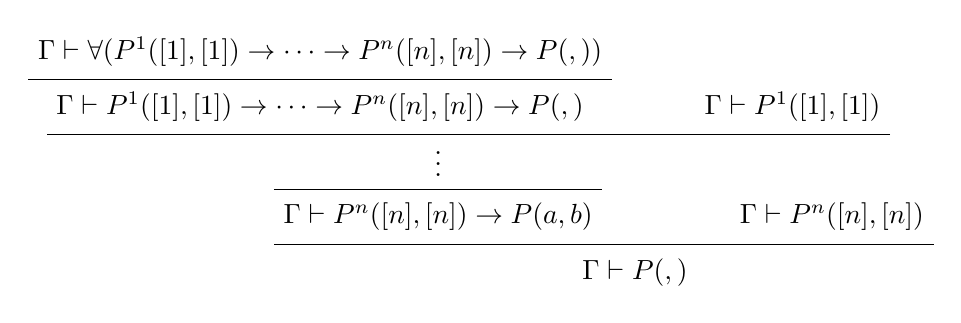
\begin{tikzpicture}[grow=up,level distance=0.7cm,
execute at begin node=$, execute at end node=$,
every node/.style={opacity=1},
every child/.style={edge from parent/.style={opacity=0}}]
\def\dist{0.7cm}
\node(e) {\Gamma\PModels  P(\predPFst,\predPSnd)} [sibling distance = 5cm]
	child {node(1) {\Gamma\PModels P^ n(\predPFst[n],\predPSnd[n])}}
	child {node(2) {\Gamma\PModels P^ n(\predPFst[n],\predPSnd[n])\to P(a,b)}
		child {{node[label={[yshift=-0.44cm]above:\vdots}](21) {}} [sibling distance = 6cm]
			child[xshift=1.5cm] {node(211) {\Gamma\PModels P^ 1(\predPFst[1],\predPSnd[1])}}
			child[xshift=1.5cm] {node(212) {\Gamma\PModels P^ 1(\predPFst[1],\predPSnd[1])\to\dots\to P^ n(\predPFst[n],\predPSnd[n])\to P(\predPFst,\predPSnd)}
				child {node(2121) {\Gamma\PModels \forall\predVec(P^ 1(\predFst[1],\predSnd[1])\to\dots\to P^n(\predFst[n],\predSnd[n])\to P(\predFst,\predSnd))}}}}};


\def\nodes{,1,2,21,211,212,2121}
\def\identifier{C1:3}
\foreach \x in \nodes{
\ifnodedefined{\x}{
	\coordinate(c\x) at (\x);
	\coordinate(\identifier.\x) at (0,0);
}{}
}
\coordinate(c) at (e);
\def\lvl{3.5mm}

%draw lines for each node with 2 children (add parents with 2 children)
\foreach \x in \nodes{
\ifnodedefined{\identifier.\x1}{
	%calculate with of line
	\getwidthofnode{\sright}{\x1}
	%if there is a right child draw wide line
	\ifnodedefined{\identifier.\x2}{
		\getwidthofnode{\sleft}{\x2}
		%draw line
		\draw[shorten <=-\sright/2, shorten >=-\sleft/2] ([yshift=-\lvl]c\x1) -- ([yshift=-\lvl]c\x2);
	} %else only one child
	{
		\ifnodedefined{\x}
			{\getwidthofnode{\sleft}{\x}}
			{\getwidthofnode{\sleft}{e}}
		%get widht corresponding to the widht of the bigger node
		\pgfmathsetlength{\sright}{max(\sright,\sleft)}
		%draw line
		\draw (c\x)+(-\sright/2,+\lvl) -- +(\sright/2,+\lvl);
	}
}{}
}
\end{tikzpicture}
	\end{figure}
	
	For $i\in\{1,\dots,n\}$ we can now apply the induction hypothesis to $\Gamma\PModels P^i(\predPFst[i],\predPSnd[i])$ and we get that there exists an $M_i$ such that $\trans{\Gamma}\lambdaModels M_i:\code{P^i}{\predPFst[i]}{\predPSnd[i]}$. Now it is easy to see that with $M:=x_A\vec{\beta}M_1\dots M_n$ the statement $M:\code{P}{\predPFst}{\predPSnd}$ is derivable from $\trans{\Gamma}$.
\end{itemize}
\end{proof}

\begin{lemma}\label{l1}
Let $\Gamma$ be a \SysP-basis such that $\Gamma\PModels\false$ holds. Then there exists a term $M\in\lambdaTerms$ such that $\trans{\Gamma}\lambdaModels M:\false$ holds.
\end{lemma}
\begin{proof}
Again we proof this by induction on the length $l$ of the proof.

\begin{itemize}
	\item[] \underline{$l=0$} It follows that $\false$ has to be deduced by the Axiom rule. So $\false\in\Gamma$ and therefore $(x_{\false}:\false)\in\trans{\Gamma}$. Now the term $M:=x_{\false}$ fulfills the condition.
	
	\item[] \underline{$l>0$} There are two ways $\false$ can be deduced in more than zero steps. 
	Firstly we could have a universal formula $A=\forall\predVec(P^1(\predFst[1],\predSnd[1])\to\dots\to P^n(\predFst[n],\predSnd[n])\to \false)$ in $\Gamma$ where $\predVec=\predVec[1]\dots\predVec[m]$ for some $m\in\N$ and some $\predVec[1],\dots,\predVec[m]\in\VarP$ and a $\vec{\beta}=\overline{\beta}_1\dots\overline{\beta}_m$ for some $\overline{\beta}_1,\dots,\overline{\beta}_m\in\VarP$. In this case we can construct $M$ as in the previous proof.%TODO rephrase


	And secondly we also could have an existential formula of the form $A=\forall\predVec(P^1(\predFst[1],\predSnd[1])\to\dots\to \forall\beta(P^n(\predFst[n],\predSnd[n])\to\false)\to \false)$ in $\Gamma$ and 
\end{itemize}
\end{proof}

In the next two lemmas we will prove the $\Leftarrow$ direction.

\begin{lemma}\label{l2h}
Let $\Gamma$ be a \SysP-basis, $M\in\lambdaTerms$, $P\in\RelP$, and $\predTFst,\predTSnd\in\lambdaTypes$ such that $\trans{\Gamma}\lambdaModels M:\code{P}{\predTFst}{\predTSnd}$ holds.
%Then $t_1=a$ and $t_2=b$ for some $a,b\in\VarP$ (remember that $\VarP\subseteq\lambdaTypVar$). Furthermore $\Gamma\PModels P(a,b)$ holds.
Then $\predTFst, \predTSnd\in\VarP$ (remember that $\VarP\subseteq\lambdaTypVar$). Furthermore $\Gamma\PModels P(\predTFst,\predTSnd)$ holds.
\end{lemma}
\begin{proof}
Note that all well typed $\lambda2$ terms are strongly normalizing (see %TODO reference
). Hence, $M$ is well typed in $\lambda2$, we can assume that $M$ is in normal form. %TODO define normal form, and typerhaltungstheorem!

We now proof the lemma by structural induction on the term $M$.
\begin{itemize}
	\item[] \underline{$M=x$} for some $y\in\lambdaValVar$.\\
		It follows that $(x:\code{P}{\predTFst}{\predTSnd})\in\trans{\Gamma}$.
		Now the definition of $\trans{\Gamma}$ yields that $P(\predTFst,\predTSnd)\in\Gamma$. Therefore $\predTFst,\predTSnd\in\VarP$ and $\Gamma\PModels P(s,t)$ holds trivially.
	\item[] \underline{$M=M_1M_2$} for some $M_1,M_2\in\lambdaTerms$.\\
		Since $M$ is in normal form we have that $M_1=xN_1\dots N_k$ for some $x\in\lambdaValVar$, $k\in\N^+$, and some $N_1,\dots,N_k\in\lambdaTerms\cup\lambdaTypes$. %TODO There is only one kind of %TODO functional neccessary P(a,b)
		%type with target | this is not a target -> $\code{P}{\alpha}{\beta}$ 
		
		It follows that $x=x_A$ and $(x:\trans{A})\in\trans{\Gamma}$ for some universal formula $A=\forall\predVec(P^1(\predFst[1],\predSnd[1])\to\dots\to P^n(\predFst[n],\predSnd[n])\to P(\predFst,\predSnd))$ in $\Gamma$ where $\predVec=\predVec[1]\dots\predVec[m]$ for some $m\in\N$ and some $\predVec[1],\dots,\predVec[m]\in\VarP$.
		%for some $P^i\in\RelP$ and some $\predFst[i], \predSnd[i]\in\VarP$ for all $i\in\{1,\dots,n\}$, $\predFst,\predSnd\in\VarP$, and $\predVec=\predVec[1]\dots\predVec[m]$ for some $\predVec[1],\dots,\predVec[m]\in\VarP$. %forall ai exists j: ai=aj or ai=bj
		
		%$\vec{\alpha}=\alpha_\mapping{1}\dots\alpha_\mapping{m}$ where $\mappingSymbol\colon \{1,\dots,m\}\to\{1,\dots,n\}$ is a mapping. %more than injective since a_v(i)=a_v(j) => i=j

		Furthermore $M=x\vec{t}\vec{N}$ for some $\predTVec=\predTVec[1]\dots \predTVec[m]$ with $\predTVec[1],\dots,\predTVec[m]\in\lambdaTypes$ and some $\vec{N}=N_1\dots N_n$ with $N_1,\dots,N_n\in\lambdaTerms$ and $\trans{\Gamma}\lambdaModels N_i:\code{P^i}{\predTFst[i]}{\predTSnd[i]}$ (where $\predTFst[i]=\predFst[i]\left[\predVec:=\predTVec\hspace{1mm}\right]$ and  $\predTSnd[i]=\predSnd[i]\left[\predVec:=\predTVec\hspace{1mm}\right]$) for $i\in\{1,\dots,n\}$.
		
		%$\vec{t}=(s,\dots,t_m)$, $A_i=P^i(\alpha_i,\beta_i)$. $x=x_A$? %TODO t_1,t_2 for 2 different variables!!!
		
		%$M=x\vec{t}\vec{N}$, $\trans{\Gamma}\lambdaModels N_i:\widetilde{A_i}$ where $\widetilde{A_i}=\trans{A_i}\left[\vec{\alpha}:=\vec{t}\hspace{1mm}\right]=\code{P^i}{\widetilde{a}_i}{\widetilde{b}_i}$ and $\widetilde{a}_i=\alpha_i\left[\vec{\alpha}:=\vec{t}\hspace{1mm}\right]$ for $i\in\{1,\dots,n\}$
		
		\begin{figure}[H]
			\centering
			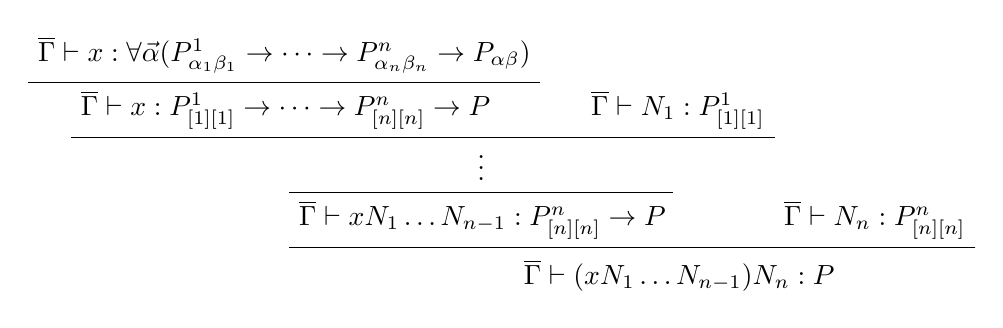
\begin{tikzpicture}[grow=up,level distance=0.7cm,
execute at begin node=$, execute at end node=$,
every node/.style={opacity=1},
every child/.style={edge from parent/.style={opacity=0}}]
\def\dist{0.7cm}
\node(e) {\trans{\Gamma}\lambdaModels (x\predTVec N_1\dots N_{n-1})N_n:\code{P}{\predTFst}{\predTSnd}} [sibling distance = 5cm]
	child {node(1) {\trans{\Gamma}\lambdaModels N_n:\code{P^n}{\predTFst[n]}{\predTSnd[n]}}}
	child {node(2) {\trans{\Gamma}\lambdaModels x\predTVec N_1\dots N_{n-1}:\code{P^n}{\predTFst[n]}{\predTSnd[n]}\to\code{P}{\predTFst}{\predTSnd}}
		child {{node[label={[yshift=-0.44cm]above:\vdots}](21) {}}
			child {node(211) {\trans{\Gamma}\lambdaModels N_1:\code{P^1}{\predTFst[1]}{\predTSnd[1]}}}
			child {node(212) {\trans{\Gamma}\lambdaModels x\predTVec:\code{P^1}{\predTFst[1]}{\predTSnd[1]}\to\dots\to\code{P^n}{\predTFst[n]}{\predTSnd[n]}\to\code{P}{\predTFst}{\predTSnd}}
				child {node(2121) {\trans{\Gamma}\lambdaModels x:\forall\vec{\alpha}(\code{P^1}{\alpha_1}{\beta_1}\to\dots\to\code{P^n}{\alpha_n}{\beta_n}\to\code{P}{\alpha}{\beta})}}}}};


\def\nodes{,1,2,21,211,212,2121}
\def\identifier{C1:2}
\foreach \x in \nodes{
\ifnodedefined{\x}{
	\coordinate(c\x) at (\x);
	\coordinate(\identifier.\x) at (0,0);
}{}
}
\coordinate(c) at (e);
\def\lvl{3.5mm}

%draw lines for each node with 2 children (add parents with 2 children)
\foreach \x in \nodes{
\ifnodedefined{\identifier.\x1}{
	%calculate with of line
	\getwidthofnode{\sright}{\x1}
	%if there is a right child draw wide line
	\ifnodedefined{\identifier.\x2}{
		\getwidthofnode{\sleft}{\x2}
		%draw line
		\draw[shorten <=-\sright/2, shorten >=-\sleft/2] ([yshift=-\lvl]c\x1) -- ([yshift=-\lvl]c\x2);
	} %else only one child
	{
		\ifnodedefined{\x}
			{\getwidthofnode{\sleft}{\x}}
			{\getwidthofnode{\sleft}{e}}
		%get widht corresponding to the widht of the bigger node
		\pgfmathsetlength{\sright}{max(\sright,\sleft)}
		%draw line
		\draw (c\x)+(-\sright/2,+\lvl) -- +(\sright/2,+\lvl);
	}
}{}
}
\end{tikzpicture}
		\end{figure}
		
		For $i\in\{1,\dots,n\}$ we can now apply the induction hypothesis to $\trans{\Gamma}\lambdaModels N_i:\code{P^i}{\predTFst[i]}{\predTSnd[i]}$ and we get that $\predTFst[i],\predTSnd[i]\in\VarP$ and that $\Gamma\PModels P^i(\predTFst[i],\predTSnd[i])$ holds.
		
		If $\predFst=\predVec[j]$ for some $j\in\{1,\dots,n\}$ then because there are no dummy quantifiers we get that $\predTFst=\predTVec[j]$. Furthermore since $\alpha\in\FV(P(\predFst,\predSnd))\setminus\FV(A)$ it follows that there exists an $i\in\{1,\dots,n\}$ such that $\predFst\in\FV(P^i(\predFst[i],\predSnd[i]))$, i.e. $\predFst=\predFst[i]$ or $\predFst=\predSnd[i]$. It follows that $\predTFst=\predTFst[i]$ or $\predTFst=\predTSnd[i]$, in both cases we get that $\predTFst\in\VarP$.
		
		If $\predFst\neq\predVec[j]$ for all $j\in\{1,\dots,n\}$ then $\predFst\in\FV(A)$ and therefore $\predTFst=\predFst$ and $\predTFst\in\VarP$.
		
		%Since there are no dummy quantifiers it follows that $\vec{t}=\vec{a}$. Either $\alpha$ is in $\vec{\alpha}$ which implies $t_1=\alpha\left[\vec{\alpha}:=\vec{t}\hspace{1mm}\right]=a$ or $\alpha$ is free then $\alpha=t_1\in\VarP$ anyway.
		For $\predTSnd$ we can make a similar argument and get that $\predTSnd\in\VarP$.
		
		Finally we have to show that $P(\predTFst,\predTSnd)$ is a semantic consequence of $\Gamma$.
		
		\begin{figure}[H]
			\centering
			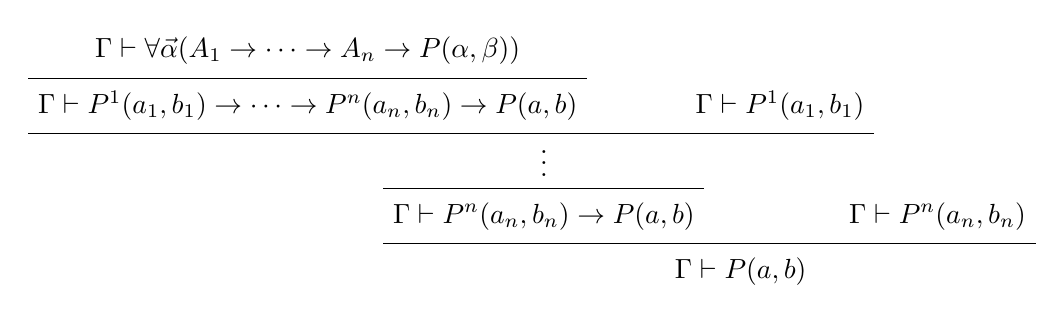
\begin{tikzpicture}[grow=up,level distance=0.7cm,
execute at begin node=$, execute at end node=$,
every node/.style={opacity=1},
every child/.style={edge from parent/.style={opacity=0}}]
\def\dist{0.7cm}
\node(e) {\Gamma\PModels  P(a,b)} [sibling distance = 5cm]
	child {node(1) {\Gamma\PModels P^ n(a_n,b_n)}}
	child {node(2) {\Gamma\PModels P^ n(a_n,b_n)\to P(a,b)}
		child {{node[label={[yshift=-0.44cm]above:\vdots}](21) {}} [sibling distance = 6cm]
			child {node(211) {\Gamma\PModels P^ 1(a_1,b_1)}}
			child {node(212) {\Gamma\PModels P^ 1(a_1,b_1)\to\dots\to P^ n(a_n,b_n)\to P(a,b)}
				child {node(2121) {\Gamma\PModels \forall\vec{\alpha}(A_1\to\dots\to A_n\to P(\alpha,\beta))}}}}};


\def\nodes{,1,2,21,211,212,2121}
\def\identifier{C1:3}
\foreach \x in \nodes{
\ifnodedefined{\x}{
	\coordinate(c\x) at (\x);
	\coordinate(\identifier.\x) at (0,0);
}{}
}
\coordinate(c) at (e);
\def\lvl{3.5mm}

%draw lines for each node with 2 children (add parents with 2 children)
\foreach \x in \nodes{
\ifnodedefined{\identifier.\x1}{
	%calculate with of line
	\getwidthofnode{\sright}{\x1}
	%if there is a right child draw wide line
	\ifnodedefined{\identifier.\x2}{
		\getwidthofnode{\sleft}{\x2}
		%draw line
		\draw[shorten <=-\sright/2, shorten >=-\sleft/2] ([yshift=-\lvl]c\x1) -- ([yshift=-\lvl]c\x2);
	} %else only one child
	{
		\ifnodedefined{\x}
			{\getwidthofnode{\sleft}{\x}}
			{\getwidthofnode{\sleft}{e}}
		%get widht corresponding to the widht of the bigger node
		\pgfmathsetlength{\sright}{max(\sright,\sleft)}
		%draw line
		\draw (c\x)+(-\sright/2,+\lvl) -- +(\sright/2,+\lvl);
	}
}{}
}
\end{tikzpicture}
		\end{figure}
		
	\item[] \underline{$M=\lambda x:t'.M'$} for some $M'\in\lambdaTerms$, some $x\in\lambdaValVar\setminus\dom(\Gamma)$, and some $t'\in\lambdaTypes$.\\
		It follows that $t'=t_1\to p_1$ and $\trans{\Gamma},(x:t_1\to p_1)\lambdaModels M':(t_2\to p_2)\to p$
		
		
		$M'=yx$; $y:(t_1\to p_1)\to(t_2\to p_2)\to p$; (eta reduction?)
		
		$M'=\lambda y:t_2\to p_2.M''$; $\Gamma,x,y \lambdaModels M''=zxy:p$
		
		\begin{figure}[H]
			\centering
			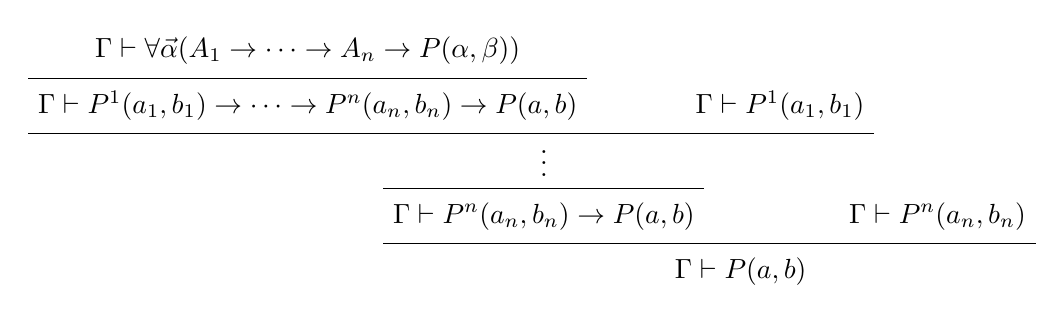
\begin{tikzpicture}[grow=up,level distance=0.7cm,
execute at begin node=$, execute at end node=$,
every node/.style={opacity=1},
every child/.style={edge from parent/.style={opacity=0}}]
\def\dist{0.7cm}
\node(e) {\Gamma\PModels  P(a,b)} [sibling distance = 5cm]
	child {node(1) {\Gamma\PModels P^ n(a_n,b_n)}}
	child {node(2) {\Gamma\PModels P^ n(a_n,b_n)\to P(a,b)}
		child {{node[label={[yshift=-0.44cm]above:\vdots}](21) {}} [sibling distance = 6cm]
			child {node(211) {\Gamma\PModels P^ 1(a_1,b_1)}}
			child {node(212) {\Gamma\PModels P^ 1(a_1,b_1)\to\dots\to P^ n(a_n,b_n)\to P(a,b)}
				child {node(2121) {\Gamma\PModels \forall\vec{\alpha}(A_1\to\dots\to A_n\to P(\alpha,\beta))}}}}};


\def\nodes{,1,2,21,211,212,2121}
\def\identifier{C1:3}
\foreach \x in \nodes{
\ifnodedefined{\x}{
	\coordinate(c\x) at (\x);
	\coordinate(\identifier.\x) at (0,0);
}{}
}
\coordinate(c) at (e);
\def\lvl{3.5mm}

%draw lines for each node with 2 children (add parents with 2 children)
\foreach \x in \nodes{
\ifnodedefined{\identifier.\x1}{
	%calculate with of line
	\getwidthofnode{\sright}{\x1}
	%if there is a right child draw wide line
	\ifnodedefined{\identifier.\x2}{
		\getwidthofnode{\sleft}{\x2}
		%draw line
		\draw[shorten <=-\sright/2, shorten >=-\sleft/2] ([yshift=-\lvl]c\x1) -- ([yshift=-\lvl]c\x2);
	} %else only one child
	{
		\ifnodedefined{\x}
			{\getwidthofnode{\sleft}{\x}}
			{\getwidthofnode{\sleft}{e}}
		%get widht corresponding to the widht of the bigger node
		\pgfmathsetlength{\sright}{max(\sright,\sleft)}
		%draw line
		\draw (c\x)+(-\sright/2,+\lvl) -- +(\sright/2,+\lvl);
	}
}{}
}
\end{tikzpicture}
		\end{figure}
	\item[] \underline{$M=\Lambda\gamma.M'$} for some $M'\in\lambdaTerms$ and some $\gamma\in\lambdaTypVar$.\\ %\setminus\FV(\Gamma)$.\\
		It follows that $\trans{\Gamma}\lambdaModels M:\forall\gamma.t'$ for some $t'\in\lambdaTypes$.
		But this can not be since $\code{P}{\predTFst}{\predTSnd}=(\predTFst\to p_1)\to(\predTSnd\to p_2)\to p$. Therefore $M$ is not of the form $\Lambda\gamma.M'$ and this case is impossible.

	\item[] \underline{$M=M'\,t'$} for some $M'\in\lambdaTerms$ and some $t'\in\lambdaTypes$.\\
		%Since $M$ is in normal form we have that either $M'=x$ for some $x\in\lambdaValVar$ and $(x:\forall\beta.t'')\in\trans{\Gamma}$ for some $\beta\in\lambdaTypVar$ and some $t''\in\lambdaTerms$ such that $t=t''\left[\beta:=t'\right]$ or $M'=xM_1\dots M_n$ for some $x\in\lambdaValVar$, $n\in\N$, and some $M_1,\dots,M_n\in\lambdaTerms\cup\lambdaTypes$.
		Since $M$ is in normal form we have that $M'=xM_1\dots M_n$ for some $x\in\lambdaValVar$, $n\in\N$, and some $M_1,\dots,M_n\in\lambdaTerms\cup\lambdaTypes$.
		Hence, $(x:\trans{A})\in\trans{\Gamma}$ for some \SysP-formula $A$ and $M=M'\,t'$, we get that this case is impossible because no such $A$ exists.
		
		The only case where the contradiction is not obvious is when $A$ is an existential formula and $M_1,\dots,M_n\in\lambdaTypes$. Furthermore because there are no dummy quantifiers $n\leq1$. So $A$ is of the form $A=\forall\predVec(P(\predFst,\predSnd))$ where $\predVec\in\{\predFst\predSnd,\predSnd\predFst,\predFst,\predSnd\}$.
		But in every case $A$ is not a \SysP-formula since there always is a $\gamma\in\FV(P(\predFst,\predSnd))\setminus\FV(A)$.
		
		%Obviously, this is impossible if $t'\notin\VarP$. But even if $t'\in\VarP$ we have a contradiction because there are no dummy quantifiers and so there is no \SysP-formula $A$ such that $\trans{A}=t''$. %TODO since the scnd condition cannot be fullfilled rephrase
\end{itemize}
\end{proof}

\begin{lemma}\label{l2}
Let $\Gamma$ be a \SysP-basis, $M\in\lambdaTerms$ such that $\trans{\Gamma}\lambdaModels M:\false$ holds. Then $\Gamma\PModels\false$ holds.
\end{lemma}
\begin{proof}
By structural induction on the term $M$.
Again we can assume that $M$ is in normal form.
\begin{itemize}
	\item[] \underline{$M=x$} for some $y\in\lambdaValVar$.\\
		It follows that $(x:\false)\in\trans{\Gamma}$. Now the definition of $\trans{\Gamma}$ yields that $\false\in\Gamma$. Therefore $\Gamma\PModels \false$ holds.
	\item[] \underline{$M=M_1M_2$} for some $M_1,M_2\in\lambdaTerms$.\\
		Because $M$ is in normal form we have that $M_1=xN_1\dots N_k$ for some $x\in\lambdaTypVar$, $k\in\N^+$, and some $N_1,\dots N_k\in\lambdaTerms\cup\lambdaTypes$.
		We know that $x=x_A$ for some $A\in\Gamma$.
		
		Firstly $A$ could be a universal formula. It follows that $A$ is of the form $A=\forall\predVec(P^1(\predFst[1],\predSnd[1])\to\dots\to P^n(\predFst[n],\predSnd[n])\to\false)$ where $\predVec=\predVec[1]\dots\predVec[m]$ for some $m\in\N$ and some $\predVec[1],\dots,\predVec[m]\in\VarP$. In this case $M=x\vec{t}\vec{N}$ for some $\predTVec=\predTVec[1]\dots \predTVec[m]$ with $\predTVec[1],\dots,\predTVec[m]\in\lambdaTypes$ and some $\vec{N}=N_1\dots N_n$ with $N_1,\dots,N_n\in\lambdaTerms$. Now $\Gamma\PModels\false$ can be deduced as in the previous proof.
		
		Secondly $A$ could be an existential formula. It follows that $A$ is of the form $A=\forall\predVec(P^1(\predFst[1],\predSnd[1])\to\dots\to \forall\beta(P^n(\predFst[n],\predSnd[n])\to\false)\to \false)$ where $\predVec=\predVec[1]\dots\predVec[m]$ for some $m\in\N$ and some $\predVec[1],\dots,\predVec[m]\in\VarP$ (w.l.o.g. $\beta\neq\predVec[i]$ for all $i\in\{1,\dots,m\}$).
		Then $M$ has to be of the form $M=x\vec{t}\vec{N}L$ for some $\predTVec=\predTVec[1]\dots \predTVec[m]$ with $\predTVec[1],\dots,\predTVec[m]\in\lambdaTypes$, some $\vec{N}=N_1\dots N_{n-1}$ with $N_1,\dots,N_{n-1}\in\lambdaTerms$, and some $L\in\lambdaTerms$. It also has to hold that $\trans{\Gamma}\lambdaModels L:\forall\beta(\code{P^n}{\predTFst[n]}{\predTSnd[n]}\to\false)$ and for $i\in\{1,\dots,n-1\}$ that $\trans{\Gamma}\lambdaModels N_i:\code{P^i}{\predTFst[i]}{\predTSnd[i]}$ (where $\predTFst[i]=\predFst[i]\left[\predVec:=\predTVec\hspace{1mm}\right]$ and  $\predTSnd[i]=\predSnd[i]\left[\predVec:=\predTVec\hspace{1mm}\right]$ for $i\in\{1,\dots,n\}$).
		
		\begin{figure}[H]
			\centering
			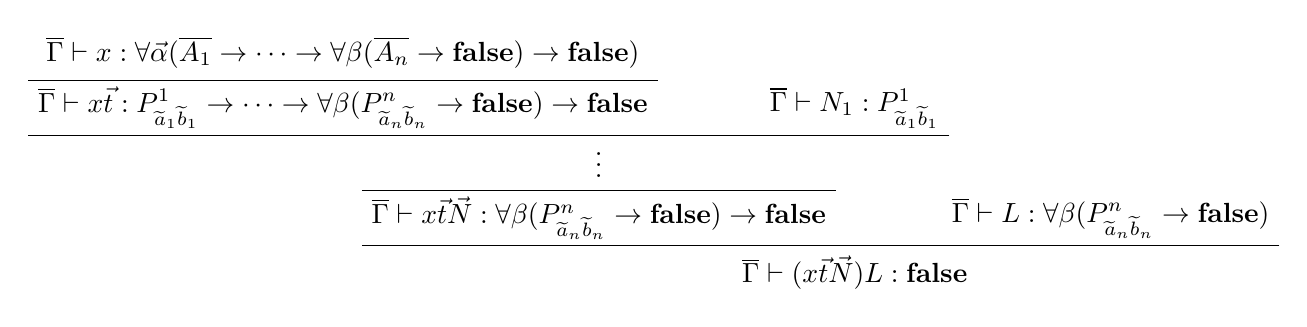
\begin{tikzpicture}[grow=up,level distance=0.7cm,
execute at begin node=$, execute at end node=$,
every node/.style={opacity=1},
every child/.style={edge from parent/.style={opacity=0}}]
\def\dist{0.7cm}
\node(e) {\trans{\Gamma}\lambdaModels (x\vec{t}\vec{N})L:\false} [sibling distance = 6.5cm]
	child {node(1) {\trans{\Gamma}\lambdaModels L:\forall\beta(\code{P^n}{\widetilde{a}_n}{\widetilde{b}_n}\to\false)}}
	child {node(2) {\trans{\Gamma}\lambdaModels x\vec{t}\vec{N}:\forall\beta(\code{P^n}{\widetilde{a}_n}{\widetilde{b}_n}\to\false)\to\false}
		child {{node[label={[yshift=-0.44cm]above:\vdots}](21) {}}
			child {node(211) {\trans{\Gamma}\lambdaModels N_1:\code{P^1}{\widetilde{a}_1}{\widetilde{b}_1}}}
			child {node(212) {\trans{\Gamma}\lambdaModels x\vec{t}:\code{P^1}{\widetilde{a}_1}{\widetilde{b}_1}\to\dots\to\forall\beta(\code{P^n}{\widetilde{a}_n}{\widetilde{b}_n}\to\false)\to\false}
				child {node(2121) {\trans{\Gamma}\lambdaModels x:\forall\vec{\alpha}(\trans{A_1}\to\dots\to\forall\beta(\trans{A_n}\to\false)\to\false)}}}}};


\def\nodes{,1,2,21,211,212,2121}
\def\identifier{C1:2}
\foreach \x in \nodes{
\ifnodedefined{\x}{
	\coordinate(c\x) at (\x);
	\coordinate(\identifier.\x) at (0,0);
}{}
}
\coordinate(c) at (e);
\def\lvl{3.5mm}

%draw lines for each node with 2 children (add parents with 2 children)
\foreach \x in \nodes{
\ifnodedefined{\identifier.\x1}{
	%calculate with of line
	\getwidthofnode{\sright}{\x1}
	%if there is a right child draw wide line
	\ifnodedefined{\identifier.\x2}{
		\getwidthofnode{\sleft}{\x2}
		%draw line
		\draw[shorten <=-\sright/2, shorten >=-\sleft/2] ([yshift=-\lvl]c\x1) -- ([yshift=-\lvl]c\x2);
	} %else only one child
	{
		\ifnodedefined{\x}
			{\getwidthofnode{\sleft}{\x}}
			{\getwidthofnode{\sleft}{e}}
		%get widht corresponding to the widht of the bigger node
		\pgfmathsetlength{\sright}{max(\sright,\sleft)}
		%draw line
		\draw (c\x)+(-\sright/2,+\lvl) -- +(\sright/2,+\lvl);
	}
}{}
}
\end{tikzpicture}
		\end{figure}
		
		For $i\in\{1,\dots,n-1\}$ we can apply Lemma \ref{l2h} to $\trans{\Gamma}\lambdaModels N_i:\code{P^i}{\predTFst[i]}{\predTSnd[i]}$ to get that $\predTFst[i],\predTSnd[i]\in\VarP$ and that $\Gamma\PModels P^i(\predTFst[i],\predTSnd[i])$.
		Now we take a closer look at $L$. First note that because either $\predFst[n]=\beta$ or there exits an $i\in\{1,\dots,n-1\}$ such that $\predFst[n]\in\FV(P^i(\predFst[i],\predSnd[i]))$ which implies that $\predTFst[n]=\predTFst[i]$ or $\predTFst[n]=\predTSnd[i]$. In both cases we get that $\predTFst[n]\in\VarP$. A similar argument yields $\predTSnd[n]\in\VarP$.
		
		$L=y$,\hspace{2cm}$A'\in\Gamma$ trivial
		
		$L=\Lambda\beta.y$,\hspace{2cm}$A'\in\Gamma$ trivial
		
		$L=\Lambda\beta.y\vec{t'}\vec{N'}$,\hspace{2cm}as in previous proof
		
		$L=\Lambda\beta.\lambda y:\code{P^n}{\predTFst[n]}{\predTSnd[n]}.N$,\hspace{2cm} $\trans{\Gamma},y:\code{P^n}{\predTFst[n]}{\predTSnd[n]}\lambdaModels N:\false$ by IH
		
		$L=\Lambda\beta.M'\,t'$, $M'=yt_1\dots t_l$,\hspace{2cm}$A'\in\Gamma$ trivial
		
		$L=M'\,t'$, $M'=yt_1\dots t_l$,\hspace{2cm}$A'\in\Gamma$ trivial
		
	\item[] \underline{$M=\lambda x:t_1.M'$} for some $M'\in\lambdaTerms$, some $x\in\lambdaValVar\setminus\dom(\Gamma)$, and some $t_1\in\lambdaTypes$.\\
		It follows that $t=t_1\to t_2$ for some $t_2\in\lambdaTypes$ which contradicts $t=\false$. So this case is impossible.

	\item[] \underline{$M=\Lambda\gamma.M'$} for some $M'\in\lambdaTerms$ and some $\gamma\in\lambdaTypVar$.\\ %\setminus\FV(\Gamma)$.\\
		It follows that $t=\forall\gamma.t'$ for some $t'\in\lambdaTypes$. Again the fact that $t=\false$ leads to a contradiction and makes this case impossible.
		

	\item[] \underline{$M=M'\,t'$} for some $M'\in\lambdaTerms$ and some $t'\in\lambdaTypes$.\\
		Since $M$ is in normal form we have that $M'=xM_1\dots M_n$ for some $x\in\lambdaValVar$, $n\in\N$, and some $M_1,\dots,M_n\in\lambdaTerms\cup\lambdaTypes$.
		Hence, $(x:\trans{A})\in\trans{\Gamma}$ for some \SysP-formula $A$ and $M=M'\,t'$, we get that this case is impossible because no such $A$ exists.
		
		%$n>0$ impossible no dummy quantifiers
		
		%$n=0$ $M'=x:\forall\alpha.\alpha$, $t'=\false$ impossible
		
\end{itemize}
\end{proof}

\begin{lemma}\label{l3}
\begin{align*}
\Gamma\PModels\false&&\text{iff}&&\text{There is a $\lambda2$ term $M$ such that } \trans{\Gamma}\lambdaModels M:\false
\end{align*}
\end{lemma}
\begin{proof}
The $\Leftarrow$ direction follows from Lemma %TODO here Lemma in Cons proof Claims
\ref{l2}. And the $\Rightarrow$ direction is proven in Lemma \ref{l1}.
\end{proof}

\begin{theorem}
\lambdaInhab{} is undecidable.
\end{theorem}
\begin{proof}
From Lemma \ref{l3} it follows that $\PCons\leq\lambdaInhab$. Since , by Theorem \ref{the:1}, \PCons{} is undecidable we have shown that \lambdaInhab{} is undecidable too.
\end{proof}
	\begin{thebibliography}{9}
\bibitem{1}
H.P. Barendregt, 1993. Lambda Calculi with Types, Handbook of Logic in Computer Science, Volume \rom{2}, 42-68.
\end{thebibliography}
	\end{sloppypar}
\end{document}
